\documentclass[conference]{IEEEtran}
\IEEEoverridecommandlockouts

% -----------------------------------------------------------------------------
% PACKAGE IMPORTS
% -----------------------------------------------------------------------------
\usepackage{amsmath,amssymb,amsfonts}
\usepackage{algorithmic}
\usepackage{graphicx}
\usepackage{textcomp}
\usepackage{xcolor}
\usepackage{booktabs}
\usepackage{tabularx}
\usepackage{multirow}
\usepackage{url}
\usepackage{cite}
\usepackage{microtype}
\usepackage{tikz}
\usetikzlibrary{shapes.geometric, arrows.meta, positioning, fit, backgrounds, calc}

\usepackage[hidelinks]{hyperref}

% -----------------------------------------------------------------------------
% TITLE & AUTHOR BLOCK
% -----------------------------------------------------------------------------
\title{SpamAdapt: Evaluating Parameter-Efficient Domain Adaptation via Full Fine-Tuning, LoRA, and DoRA for Robust SMS Scam Detection}

\author{
    \IEEEauthorblockN{Akash Uchachariya\IEEEauthorrefmark{1}, Umang Mori\IEEEauthorrefmark{1}, and Keval Bamarotiya\IEEEauthorrefmark{1}}
    \IEEEauthorblockA{\IEEEauthorrefmark{1}Department of Computer Science and Engineering\\
    [Institution / University Name Placeholder], [City, Country Placeholder]\\
    Email: \{[akash.uchachariya], [umang.mori], [keval.bamarotiya]\}@institution.edu Placeholder}
}

\begin{document}

\maketitle

% -----------------------------------------------------------------------------
% ABSTRACT
% -----------------------------------------------------------------------------
\begin{abstract}
Short Message Service (SMS) remains a critical telecommunications channel for high-priority transaction confirmations, one-time passwords (OTPs), and utility notices. However, mobile messaging has concurrently become a primary attack surface for social engineering, financial fraud, and credential phishing. Conventional SMS spam classifiers trained on legacy corpora—most notably the 2011 UCI SMS Spam Collection—suffer from severe domain shift when deployed in modern ecosystems: because legacy benign messages consist predominantly of personal social conversations, fine-tuned transformer models learn spurious correlations on transaction identifiers, customer support phone numbers, and urgent imperatives, misclassifying genuine banking and telecom alerts as spam with over 99.8\% false confidence. In this work, we present \textbf{SpamAdapt}, a comprehensive empirical study and software framework investigating parameter-efficient domain adaptation for SMS scam detection. We adapt pretrained bidirectional transformer representations (\texttt{google-bert/bert-base-uncased}, 109.5M parameters) across three regimes: Full Fine-Tuning, Low-Rank Adaptation (LoRA, $r=8$), and Weight-Decomposed Low-Rank Adaptation (DoRA, $r=8$). Using a domain-augmented retraining corpus and piecewise constrained threshold optimization, SpamAdapt recovers legitimate transactional notifications without brittle keyword overrides. Across the preserved in-distribution UCI test split ($N=774$), all models maintain over 98.0\% accuracy and 99.2\% legitimate specificity, confirming retention of foundation language capabilities. On an independent, frozen 220-message external benchmark spanning 11 categories with a four-tier provenance audit, Full Fine-Tuning achieves 87.73\% accuracy, while DoRA and LoRA achieve 77.73\% and 76.82\% accuracy while updating fewer than 0.3\% of model parameters (314.8K and 296.5K) and reducing serialized adapter storage by 99.55\% (1.82--1.90~MB vs. 418.35~MB). We show that extending training across multiple epochs causes validation-loss divergence and false-positive regressions, establishing our remediated checkpoint (\texttt{lora\_v3}) as the optimal production candidate. Finally, we implement an operational three-tier abstention framework to route borderline scores to human review, evaluate adversarial stability across 40 controlled perturbations, and deploy an interactive, privacy-preserving Streamlit web dashboard operating entirely in volatile memory.
\end{abstract}

% -----------------------------------------------------------------------------
% KEYWORDS
% -----------------------------------------------------------------------------
\begin{IEEEkeywords}
SMS scam detection, domain adaptation, Parameter-Efficient Fine-Tuning (PEFT), Low-Rank Adaptation (LoRA), Weight-Decomposed Low-Rank Adaptation (DoRA), BERT, false positive mitigation, abstention policy, natural language processing.
\end{IEEEkeywords}

% -----------------------------------------------------------------------------
% SECTION I: INTRODUCTION & MOTIVATION
% -----------------------------------------------------------------------------
\section{Introduction and Motivation}
\label{sec:intro}

Short Message Service (SMS) telecommunications continues to serve as an indispensable global communications backbone. Owing to its platform agnosticism, universal carrier interoperability, and independence from data connectivity, SMS is the default mechanism for time-critical two-factor authentication (2FA) one-time passwords (OTPs), financial transaction confirmations, parcel delivery tracking, and emergency civic broadcasts. Simultaneously, mobile messaging has emerged as the premier attack vector for financially motivated cybercrime. Modern smishing (SMS phishing) attacks have evolved far beyond early-2000s lottery schemes, adopting sophisticated social engineering tactics including Unified Payments Interface (UPI) payment collect fraud, fake electricity power disconnection warnings, bank account deactivation threats, and counterfeit application (APK) distribution~\cite{almeida2011sms,trai2018tcccpr}.

Automating SMS spam detection involves distinct linguistic and structural challenges compared to email filtering. SMS messages are constrained in sequence length (typically 160 characters per standard PDU), exhibit severe class imbalance, and frequently contain non-standard abbreviations, phonetic transliterations, and evasion orthography~\cite{delany2012sms}. Historically, machine learning systems relied on hand-crafted lexical features paired with classical classifiers such as Naive Bayes, Support Vector Machines (SVMs), and Random Forests~\cite{almeida2011sms}. While these models achieved high accuracy on static datasets, they lacked bidirectional contextual understanding and degraded rapidly on out-of-vocabulary tokens.

The emergence of pretrained language models (PLMs) based on the Transformer architecture~\cite{vaswani2017attention}, particularly Bidirectional Encoder Representations from Transformers (BERT)~\cite{devlin2019bert}, revolutionized text classification by encoding rich semantic, syntactic, and contextual representations through self-attention. Consequently, fine-tuning BERT on domain-specific classification tasks routinely establishes state-of-the-art benchmarks.

\subsection{The Legacy Dataset Disconnect and Domain Shift}
Despite the rapid evolution of mobile threat vectors, academic literature and benchmark evaluations remain tethered to corpora collected over a decade ago. The predominant benchmark, the 2011 UCI SMS Spam Collection~\cite{almeida2011sms}, exhibits two structural distributional skews:
\begin{enumerate}
    \item \textbf{Legitimate (HAM) Distribution}: Over 95\% of legitimate messages represent informal social dialogue between private individuals (e.g., \textit{``Where are you?'', ``Love you, see you tomorrow''}). Modern structured transactional notifications from commercial banks, airlines, e-commerce platforms, and government agencies are completely unrepresented.
    \item \textbf{Spam Distribution}: Malicious messages consist almost exclusively of legacy UK premium-rate ringtone subscriptions and lottery claims. Modern smishing techniques—such as urgent bank KYC update deadlines and malicious APK download links—are entirely absent.
\end{enumerate}

When deep contextual encoders like BERT are fine-tuned on this legacy distribution, they develop severe spurious correlations. Specifically, the attention layers learn to associate numerical identifiers, currency amounts, uppercase imperatives, customer care phone numbers, and hyperlinks almost exclusively with the spam class. In operational telecommunications, a false positive (filtering a legitimate bank transaction confirmation or carrier notice) is vastly more disruptive than a false negative: it locks consumers out of financial accounts, delays emergency dispatches, and erodes subscriber trust~\cite{delany2012sms}. Our empirical baseline audit revealed that standard fine-tuned models misclassified verified legitimate telecommunication notices as spam with over 99.8\% confidence.

\subsection{Computational and Parameter Constraints}
While Full Fine-Tuning updates all underlying parameters of a foundation model ($109.5\times 10^6$ parameters for BERT-base), saving and serving independent checkpoints of over 400~MB per task introduces unsustainable operational overhead in multi-tenant cloud gateways and storage-constrained mobile edge environments. Parameter-Efficient Fine-Tuning (PEFT) has emerged as an attractive solution. Low-Rank Adaptation (LoRA)~\cite{hu2022lora} freezes the foundation model and injects trainable rank decomposition matrices into the multi-head attention projections, updating fewer than 0.3\% of parameters. Weight-Decomposed Low-Rank Adaptation (DoRA)~\cite{liu2024dora} decouples weight magnitude from directional updates to bridge the optimization gap between full fine-tuning and low-rank adaptation.

In this paper, we present \textbf{SpamAdapt}, an empirical investigation evaluating Full Fine-Tuning, LoRA, and DoRA under identical, CPU-bounded experimental conditions. We investigate domain adaptation on an augmented multi-tier dataset, evaluate models across an independent external benchmark ($N=220$), analyze multi-epoch overfitting dynamics, and deploy an operational three-tier abstention framework integrated into an interactive Streamlit web dashboard.

% -----------------------------------------------------------------------------
% SECTION II: PROBLEM STATEMENT & RESEARCH OBJECTIVES
% -----------------------------------------------------------------------------
\section{Problem Statement and Research Objectives}
\label{sec:problem_objectives}

\subsection{Problem Formulation}
Let $\mathcal{X}$ denote the space of raw text messages, and let $\mathcal{Y} = \{0, 1\}$ denote the binary ground-truth space, where $y=0$ corresponds to legitimate communication ($\text{HAM}$) and $y=1$ denotes unsolicited or fraudulent communication ($\text{SPAM}$). Given an input token sequence $\mathbf{x} = (x_1, x_2, \dots, x_T) \in \mathcal{X}$ bounded by a maximum sequence length $T \le 128$, a contextual transformer encoder parameterized by initial weights $\Theta_0 \in \mathbb{R}^D$ computes a sequence representation $\mathbf{h} = \mathcal{M}(\mathbf{x}; \Theta)$. Downstream sequence classification applies a parameter update $\Delta \Theta$ to yield task-adapted parameters $\Theta^* = \Theta_0 + \Delta \Theta$, producing classification logits $\mathbf{z} = (z_{\text{ham}}, z_{\text{spam}}) \in \mathbb{R}^2$ and normalized class probabilities via the softmax function:
\begin{equation}
    P(y = 1 \mid \mathbf{x}) = \frac{\exp(z_{\text{spam}})}{\exp(z_{\text{ham}}) + \exp(z_{\text{spam}})}.
    \label{eq:softmax}
\end{equation}

The primary engineering challenge is to determine parameter updates $\Delta \Theta$ that minimize cross-entropy loss on target distributions while updating only a minute parameter fraction $\Delta \Theta \ll \Theta_0$, preventing catastrophic false positives on high-value transactional communications without introducing manual keyword heuristics.

\subsection{Research Objectives}
SpamAdapt was organized around five core scientific objectives:
\begin{enumerate}
    \item \textbf{Empirical PEFT Comparison}: Systematically compare Full Fine-Tuning, LoRA, and DoRA on identical architectures and data splits, quantifying trade-offs in predictive quality, parameter count, disk footprint, CPU training time, and per-message inference latency.
    \item \textbf{Mitigation of Spurious False Positives}: Engineer an augmented domain-adaptation training procedure and a validation-tuned piecewise decision threshold to eliminate false positives on structured banking and telecom notifications.
    \item \textbf{Zero-Leakage Benchmark Evaluation}: Evaluate all adapted models across an independent 220-message external benchmark spanning 11 real-world categories, accompanied by a transparent four-tier provenance audit.
    \item \textbf{Overfitting and Convergence Auditing}: Empirically document multi-epoch training dynamics to analyze why validation loss diverges after minimal epochs and formalize the selection of our remediated checkpoint (\texttt{lora\_v3}).
    \item \textbf{Uncertainty Quantification and Deployment}: Formulate an operational three-tier abstention framework to route ambiguous inputs to human review, evaluate adversarial surface stability, and deploy an end-to-end web dashboard operating under strict volatile memory privacy.
\end{enumerate}

% -----------------------------------------------------------------------------
% SECTION III: RELATED WORK
% -----------------------------------------------------------------------------
\section{Related Work}
\label{sec:related_work}

\subsection{Classical SMS Spam Filtering}
Early investigations in SMS spam filtering focused on feature extraction and shallow machine learning. Almeida et al.~\cite{almeida2011sms} introduced the canonical UCI SMS Spam Collection, comparing Naive Bayes, Support Vector Machines, and decision trees. Delany et al.~\cite{delany2012sms} surveyed mobile spam filtering techniques, highlighting the critical operational asymmetry: legitimate false alarms impose severe user friction compared to uncaught spam. Subsequent efforts explored $n$-gram representations, character-level TF-IDF, and recurrent architectures such as Long Short-Term Memory (LSTM) networks~\cite{hochreiter1997lstm}. However, bag-of-words and shallow embeddings fail to capture long-range contextual relationships, syntactic inversion, and adversarial token modifications.

\subsection{Transformer Language Models in Text Classification}
The Transformer self-attention architecture~\cite{vaswani2017attention} catalyzed modern NLP. Devlin et al.~\cite{devlin2019bert} established the Bidirectional Encoder Representations from Transformers (BERT), pretrained via masked language modeling and next-sentence prediction. Subsequent variants, including RoBERTa~\cite{liu2019roberta} and DeBERTa~\cite{he2020deberta}, demonstrated that bidirectional contextual representations generalize effectively across benchmark tasks. Fine-tuning BERT for sequence classification by appending a linear projection head to the pooled \texttt{[CLS]} representation became the standard paradigm for NLP benchmarks~\cite{wang2018glue}.

\subsection{Parameter-Efficient Fine-Tuning (PEFT)}
As foundational models scaled from millions to hundreds of billions of parameters, full parameter updates became computationally prohibitive~\cite{ding2023peft_nature}. PEFT approaches address this challenge by updating only a small parameter subset:
\begin{itemize}
    \item \textbf{Addition-based Methods}: Insert lightweight trainable adapter blocks between transformer layers (Houlsby et al.~\cite{houlsby2019adapter}; Pfeiffer et al.~\cite{pfeiffer2021adapterfusion}) or prepend learnable virtual prompt tokens to inputs (Prefix-Tuning~\cite{li2021prefix}; Prompt-Tuning~\cite{lester2021prompt}).
    \item \textbf{Specification-based Methods}: Fine-tune selected inherent model parameters while freezing others. BitFit (Ben Zaken et al.~\cite{zaken2022bitfit}) optimizes only bias terms, demonstrating competitive performance on select tasks.
    \item \textbf{Reparameterization Methods}: Model parameter updates as low-rank projections based on the intrinsic rank hypothesis. Hu et al.~\cite{hu2022lora} introduced Low-Rank Adaptation (LoRA), parameterizing weight deltas as the product of two low-rank matrices. AdaLoRA (Zhang et al.~\cite{zhang2023adalora}) introduces adaptive singular value pruning to allocate parameter budgets dynamically across layers. Recently, Mao et al.~\cite{mao2024dora_dynamic} proposed Dynamic LoRA (DoRA), decomposing LoRA layers into single-rank components pruned via an exponential moving average of Frobenius norms. In parallel, Liu et al.~\cite{liu2024dora} proposed Weight-Decomposed Low-Rank Adaptation (DoRA), decomposing pre-trained weights into magnitude and directional components. In this work, our PEFT implementation uses Liu et al.'s weight-decomposed DoRA formulation via Hugging Face PEFT~\cite{peft2022}, benchmarked directly against standard LoRA and full fine-tuning.
\end{itemize}

% -----------------------------------------------------------------------------
% SECTION IV: THEORETICAL FOUNDATIONS
% -----------------------------------------------------------------------------
\section{Theoretical Foundations: BERT, Full Fine-Tuning, LoRA, and DoRA}
\label{sec:theory}

\subsection{Transformer Multi-Head Self-Attention}
SpamAdapt is built upon \texttt{google-bert/bert-base-uncased}~\cite{devlin2019bert}, comprising $L = 12$ transformer encoder layers, a hidden dimension of $d_{\text{model}} = 768$, $h = 12$ self-attention heads (head dimension $d_k = d_v = 64$), and a feed-forward intermediate dimension of $d_{\text{ffn}} = 3072$, totaling $109,483,778$ parameters.

For an input sequence $\mathbf{X} \in \mathbb{R}^{T \times d_{\text{model}}}$, multi-head attention projects $\mathbf{X}$ into Query, Key, and Value representations using projection matrices $W_q, W_k, W_v \in \mathbb{R}^{d_{\text{model}} \times d_{\text{model}}}$. For each head $i \in \{1, \dots, h\}$:
\begin{equation}
    \text{head}_i = \text{Softmax}\left( \frac{(\mathbf{X}W_q^i)(\mathbf{X}W_k^i)^\top}{\sqrt{d_k}} \right)(\mathbf{X}W_v^i),
    \label{eq:attention}
\end{equation}
which are concatenated and multiplied by an output projection matrix $W_o \in \mathbb{R}^{d_{\text{model}} \times d_{\text{model}}}$:
\begin{equation}
    \text{MHA}(\mathbf{X}) = \text{Concat}(\text{head}_1, \dots, \text{head}_h)W_o.
    \label{eq:mha}
\end{equation}

For classification, the special token representation $\mathbf{h}_{[\text{CLS}]} \in \mathbb{R}^{768}$ is extracted from the 12th transformer block and passed to a linear classification head:
\begin{equation}
    \mathbf{z} = \mathbf{h}_{[\text{CLS}]} W_{\text{head}} + \mathbf{b}_{\text{head}},
    \label{eq:cls_head}
\end{equation}
where $W_{\text{head}} \in \mathbb{R}^{768 \times 2}$ and $\mathbf{b}_{\text{head}} \in \mathbb{R}^2$.

\subsection{Full Fine-Tuning}
In Full Fine-Tuning, all pretrained parameter matrices $W_0 \in \mathbb{R}^{d \times k}$ across all self-attention, feed-forward, layer normalization, and classification layers are updated during backpropagation:
\begin{equation}
    W = W_0 + \Delta W.
    \label{eq:full_ft}
\end{equation}
While unconstrained fine-tuning provides maximum modeling capacity, updating all 109.5M parameters requires saving 418.35~MB per task checkpoint and risks catastrophic forgetting on generic language distributions.

\subsection{Low-Rank Adaptation (LoRA)}
LoRA~\cite{hu2022lora} hypothesizes that the weight updates $\Delta W$ possess a low intrinsic rank during task adaptation. For a frozen pretrained weight matrix $W_0 \in \mathbb{R}^{d \times k}$, LoRA parameterizes $\Delta W$ as the product of two low-rank matrices $B \in \mathbb{R}^{d \times r}$ and $A \in \mathbb{R}^{r \times k}$, where the rank $r \ll \min(d, k)$:
\begin{equation}
    W = W_0 + \Delta W = W_0 + \frac{\alpha}{r} B \cdot A.
    \label{eq:lora}
\end{equation}
Here, matrix $A$ is initialized from a zero-mean Gaussian distribution $\mathcal{N}(0, \sigma^2)$, and matrix $B$ is initialized to zero, ensuring $\Delta W = 0$ at the onset of training. The scalar $\alpha$ is a constant scaling hyperparameter. In SpamAdapt, we configure $r = 8$ and $\alpha = 16$, applying adapters to the query ($W_q$) and value ($W_v$) projection matrices of all 12 self-attention layers:
\begin{equation}
    N_{\text{trainable}} = 2 \times L \times (d_{\text{model}} \times r + r \times d_{\text{model}}) + N_{\text{head}},
\end{equation}
yielding exactly $296,450$ trainable parameters (0.270\% of the foundation model). At inference time, the low-rank update can be merged into $W_0$ statically ($W = W_0 + \frac{\alpha}{r}BA$), incurring zero additional latency overhead.

\subsection{Weight-Decomposed Low-Rank Adaptation (DoRA)}
DoRA (Liu et al.~\cite{liu2024dora}) bridges the architectural capacity gap between full fine-tuning and LoRA by decomposing weight matrices into magnitude and directional components. Mathematically, any weight matrix $W \in \mathbb{R}^{d \times k}$ can be reparameterized as:
\begin{equation}
    W = m \odot \frac{V}{\|V\|_c},
    \label{eq:dora_decomp}
\end{equation}
where $m \in \mathbb{R}^{1 \times k}$ is a learnable magnitude vector, $\|\cdot\|_c$ denotes the column-wise vector norm, $\odot$ denotes element-wise broadcasting multiplication, and $V \in \mathbb{R}^{d \times k}$ represents the directional matrix.

DoRA initializes the magnitude vector to the norm of the frozen pretrained weights, $m = \|W_0\|_c$, and parameterizes the directional component using low-rank adapter matrices:
\begin{equation}
    W = m \odot \frac{W_0 + \Delta W}{\|W_0 + \Delta W\|_c} = m \odot \frac{W_0 + \frac{\alpha}{r}BA}{\|W_0 + \frac{\alpha}{r}BA\|_c}.
    \label{eq:dora}
\end{equation}
By decoupling magnitude optimization from directional updates, DoRA allows gradient descent to alter the directional orientation of weight matrices without destabilizing their scale. DoRA adds $18,432$ trainable magnitude parameters ($12 \text{ layers} \times 2 \text{ projections} \times 768$ dimensions) over standard LoRA, resulting in $314,882$ trainable parameters (0.287\%). However, because directional normalization is computed dynamically during the forward pass, DoRA introduces a modest runtime latency overhead on CPU execution.

\begin{table}[t]
\caption{Mathematical Comparison of Adaptation Paradigms}
\label{tab:paradigm_comparison}
\centering
\begin{tabularx}{\columnwidth}{lXcc}
\toprule
\textbf{Method} & \textbf{Weight Formulation ($W$)} & \textbf{Trainable Params} & \textbf{Storage} \\
\midrule
Full FT & $W_0 + \Delta W$ & $109,483,778$ & 418.35~MB \\
LoRA & $W_0 + \frac{\alpha}{r}BA$ & $296,450$ & 1.82~MB \\
DoRA & $m \odot \frac{W_0 + \frac{\alpha}{r}BA}{\|W_0 + \frac{\alpha}{r}BA\|_c}$ & $314,882$ & 1.90~MB \\
\bottomrule
\end{tabularx}
\end{table}

% -----------------------------------------------------------------------------
% SECTION V: SPAMADAPT SYSTEM ARCHITECTURE
% -----------------------------------------------------------------------------
\section{SpamAdapt System Architecture}
\label{sec:system_arch}

The SpamAdapt inference pipeline operates as an end-to-end, modular five-stage software architecture designed for predictable, low-latency execution on CPU hardware, illustrated in Fig.~\ref{fig:architecture}.

\begin{figure}[t]
\centering
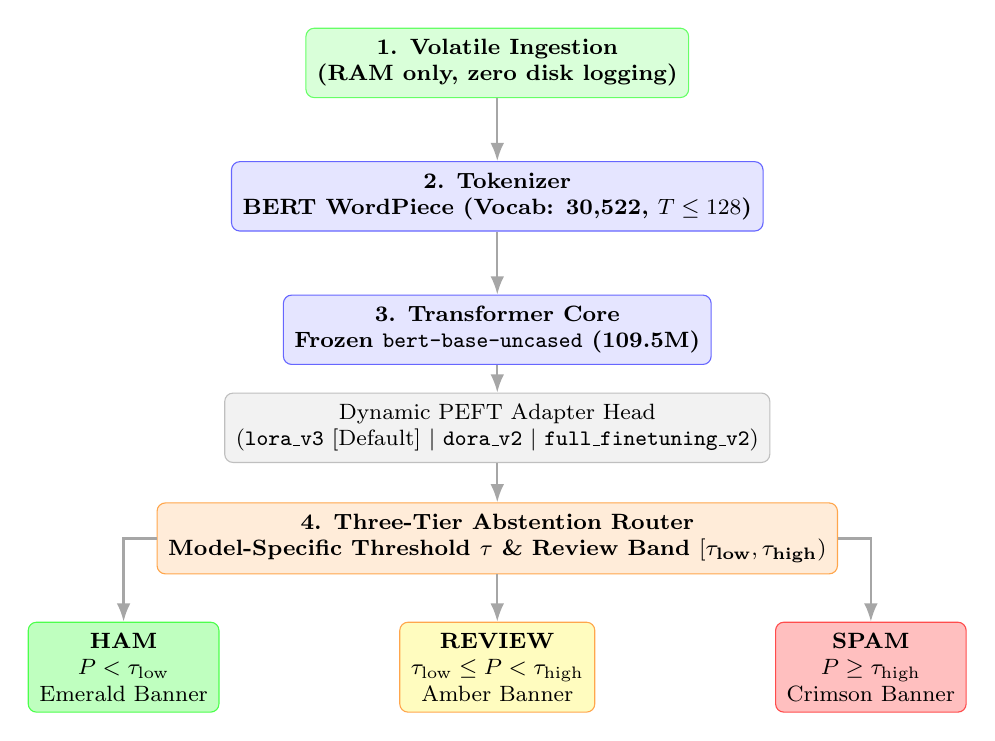
\begin{tikzpicture}[
    node distance=0.8cm and 0.5cm,
    base/.style={draw, rounded corners=3pt, align=center, font=\footnotesize, minimum height=0.65cm, inner sep=4pt},
    stage/.style={base, fill=blue!10, draw=blue!60, font=\bfseries\footnotesize},
    sub/.style={base, fill=gray!10, draw=gray!50},
    decision/.style={base, fill=orange!15, draw=orange!70, font=\bfseries\footnotesize},
    arrow/.style={-Latex, thick, draw=gray!70}
]

% Nodes
\node[stage, fill=green!15, draw=green!60] (input) {1. Volatile Ingestion\\(RAM only, zero disk logging)};
\node[stage, below=of input] (tok) {2. Tokenizer\\BERT WordPiece (Vocab: 30,522, $T \le 128$)};
\node[stage, below=of tok] (core) {3. Transformer Core\\Frozen \texttt{bert-base-uncased} (109.5M)};
\node[sub, below=0.35cm of core, minimum width=6cm] (adapters) {Dynamic PEFT Adapter Head\\(\texttt{lora\_v3} [Default] $\mid$ \texttt{dora\_v2} $\mid$ \texttt{full\_finetuning\_v2})};
\node[decision, below=0.5cm of adapters] (routing) {4. Three-Tier Abstention Router\\Model-Specific Threshold $\tau$ \& Review Band $[\tau_{\text{low}}, \tau_{\text{high}})$};

% Outputs
\node[base, fill=green!25, draw=green!70, below left=0.6cm and -0.8cm of routing] (ham) {\textbf{HAM}\\$P < \tau_{\text{low}}$\\Emerald Banner};
\node[base, fill=yellow!25, draw=orange!70, below=0.6cm of routing] (review) {\textbf{REVIEW}\\$\tau_{\text{low}} \le P < \tau_{\text{high}}$\\Amber Banner};
\node[base, fill=red!25, draw=red!70, below right=0.6cm and -0.8cm of routing] (spam) {\textbf{SPAM}\\$P \ge \tau_{\text{high}}$\\Crimson Banner};

% Arrows
\draw[arrow] (input) -- (tok);
\draw[arrow] (tok) -- (core);
\draw[arrow] (core) -- (adapters);
\draw[arrow] (adapters) -- (routing);
\draw[arrow] (routing) -| (ham);
\draw[arrow] (routing) -- (review);
\draw[arrow] (routing) -| (spam);

\end{tikzpicture}
\caption{SpamAdapt End-to-End System Architecture. Raw inputs are processed exclusively in volatile RAM. Dynamic adapter heads project representations to calibrated logits, which are routed via model-specific thresholds and abstention bands.}
\label{fig:architecture}
\end{figure}

\begin{enumerate}
    \item \textbf{Volatile Ingestion Stage}: Raw SMS text is received via HTTP API or user input. To uphold strict telecommunication privacy, strings are held strictly in volatile RAM. No intermediate database tables, debug files, or cloud telemetry persist user message strings to disk.
    \item \textbf{Tokenization Stage}: The input sequence is processed by the BERT WordPiece tokenizer, inserting special tokens \texttt{[CLS]} and \texttt{[SEP]}. Inputs exceeding 128 tokens are truncated, and shorter inputs are padded to the batch length.
    \item \textbf{Transformer Core Stage}: The tokenized tensors pass through the frozen \texttt{bert-base-uncased} backbone. Dynamic PyTorch hooks inject the selected adaptation matrices into self-attention projections. Model checkpoints are cached in memory using Streamlit's \texttt{@st.cache\_resource} decorator.
    \item \textbf{Decision Routing Stage}: Model logits are converted to class probabilities via softmax. Predictions are evaluated against a model-specific threshold $\tau$ and routed through our three-tier abstention policy.
    \item \textbf{Presentation Stage}: Results are visualized via a Streamlit web application featuring color-coded status banners, diagnostic expanders, and volatile session history.
\end{enumerate}

% -----------------------------------------------------------------------------
% SECTION VI: DATASET & PREPROCESSING
% -----------------------------------------------------------------------------
\section{Dataset Architecture, Preprocessing, and Provenance}
\label{sec:dataset}

\subsection{In-Distribution Baseline Corpus (UCI SMS)}
The foundational training and testing corpus was constructed from the raw UCI SMS Spam Collection~\cite{almeida2011sms}, containing 5,574 messages. Preprocessing executed strict deduplication: 414 duplicate records were removed, yielding exactly 5,160 clean unique messages (4,518 HAM, 642 SPAM).

The cleaned dataset was partitioned using stratified sampling into a canonical 70\%/15\%/15\% split, verified via cryptographic SHA-256 hashes recorded in \texttt{baseline\_manifest.json}:
\begin{itemize}
    \item \textbf{Training Split}: 3,612 samples (3,163 HAM, 449 SPAM; SHA-256: \texttt{1278901b...}).
    \item \textbf{Validation Split}: 774 samples (678 HAM, 96 SPAM; SHA-256: \texttt{79e31eb3...}).
    \item \textbf{Preserved Test Split}: 774 samples (677 HAM, 97 SPAM; SHA-256: \texttt{75d4e112...}).
\end{itemize}

\subsection{Domain-Augmented Corpus (v2 Retraining)}
To mitigate the baseline failure on structured transactional messages, we curated an augmented pool of **140 modern enterprise and smishing messages** (80 HAM, 60 SPAM) spanning 10 domain categories: telecom service notices, bank OTPs, UPI transaction confirmations, courier delivery tracking, urgent utility disconnection phishing, KYC deactivation threats, fake loan/lottery scams, and Hinglish code-mixed fraud.

Using cluster-aware stratified sampling, the 140 curated messages were integrated with the baseline splits to form the v2 retraining corpus:
\begin{itemize}
    \item \textbf{Augmented Train Split}: 3,190 samples (UCI Train subset + 94 curated messages).
    \item \textbf{Augmented Validation Split}: 562 samples (UCI Val subset + 46 curated messages).
\end{itemize}
A cross-split audit confirmed zero sample overlap or template leakage between the augmented training and validation partitions.

\subsection{Independent External Benchmark v2 ($N=220$)}
To evaluate true out-of-domain generalization without data snooping, we constructed an independent benchmark of **220 samples** (110 HAM, 110 SPAM) across 11 balanced categories (Table~\ref{tab:benchmark_categories}). To ensure complete academic transparency, all 220 samples are audited under a **four-tier provenance hierarchy**:
\begin{enumerate}
    \item \textbf{Regulatory Advisory Exhibits (50.0\%, 110 samples)}: Authentic scam exhibits sourced from official cybercrime advisories published by the Reserve Bank of India (RBI), Telecom Regulatory Authority of India (TRAI), Press Information Bureau (PIB), and Indian Computer Emergency Response Team (CERT-In).
    \item \textbf{Enterprise Templates Redacted (38.6\%, 85 samples)}: Authentic transactional notification templates with customer PII synthetically redacted.
    \item \textbf{Verified Real-World Mobile Captures (6.8\%, 15 samples)}: Consented, verified mobile SMS captures gathered directly from personal consumer devices.
    \item \textbf{Contrastive Synthetic Pairs (4.5\%, 10 samples)}: Minimal lexical edits isolating specific smishing cues.
\end{enumerate}

An automated leakage audit confirmed **0 exact matches** and **0 normalized lexical leaks** between the external benchmark and any training or validation split.

\begin{table}[t]
\caption{Composition of External Benchmark ($N=220$)}
\label{tab:benchmark_categories}
\centering
\begin{tabularx}{\columnwidth}{lXcc}
\toprule
\textbf{Category} & \textbf{Class} & \textbf{Samples} & \textbf{Core Linguistic Focus} \\
\midrule
Personal Conversation & HAM & 15 & Informal interpersonal social chat \\
Appointment / Account & HAM & 15 & Routine service and schedule alerts \\
Telecom Service & HAM & 15 & Mobile reverification, plan updates \\
Bank OTP Notification & HAM & 15 & Mandatory 2FA codes, login alerts \\
Delivery Tracking & HAM & 15 & Courier and logistics shipping links \\
UPI Transaction Alert & HAM & 25 & Debit/credit balance alerts, ref IDs \\
Legitimate Promotional & HAM & 10 & Merchant offers (Zomato, Swiggy) \\
Phishing / Credential & SPAM & 25 & Counterfeit netbanking portal URLs \\
KYC Account Blocking & SPAM & 25 & Urgent PAN deactivation threats \\
Fake Jobs / Loans & SPAM & 45 & Instant loan and lottery lures \\
Hinglish Code-Mixed & SPAM & 15 & Romanized Hindi smishing scripts \\
\bottomrule
\end{tabularx}
\end{table}

% -----------------------------------------------------------------------------
% SECTION VII: EXPERIMENTAL METHODOLOGY
% -----------------------------------------------------------------------------
\section{Experimental Methodology}
\label{sec:methodology}

\subsection{Training Environment and Hardware}
All fine-tuning and benchmarking experiments were conducted on x86\_64 multi-core CPU architectures running Windows 11 AMD64, utilizing PyTorch 2.1.2+cpu, Hugging Face Transformers 4.36+, and PEFT 0.21.2. CUDA hardware acceleration was genuinely unavailable; consequently, all recorded training times and inference latencies represent reproducible CPU execution.

\subsection{Hyperparameter Optimization}
To prevent overfitting on the compact augmented dataset pool, all v2 models were trained for exactly **1 training epoch** with the following hyperparameters:
\begin{itemize}
    \item \textbf{Loss Function}: Binary Cross-Entropy (\texttt{nn.CrossEntropyLoss}).
    \item \textbf{Optimizer}: \texttt{AdamW}~\cite{loshchilov2019adamw} ($\beta_1 = 0.9, \beta_2 = 0.999$, weight decay $\lambda = 0.01$).
    \item \textbf{Learning Rates}: $\eta = 2 \times 10^{-5}$ for Full Fine-Tuning; $\eta = 2 \times 10^{-4}$ for LoRA and DoRA.
    \item \textbf{Batch Size}: Physical mini-batch size = 2, gradient accumulation steps = 4 (effective batch size = 8).
    \item \textbf{Sequence Length}: $T_{\max} = 128$ tokens.
\end{itemize}

\subsection{Piecewise Constrained Threshold Optimization}
Rather than assuming an uncalibrated default threshold of $\tau = 0.50$, decision thresholds were optimized strictly on \texttt{augmented\_val.csv} ($N=562$) using a piecewise objective function designed to heavily penalize false alarms on legitimate communications:
\begin{equation}
    \text{Score}(\tau) = 
    \begin{cases} 
        F_{1,\text{macro}} + 0.1 \times R_{\text{HAM}}, & \text{if } R_{\text{HAM}} \ge 0.98 \\ 
        F_{1,\text{macro}} - 5.0 \times (0.98 - R_{\text{HAM}}), & \text{if } R_{\text{HAM}} < 0.98 
    \end{cases}
    \label{eq:threshold_opt}
\end{equation}
The resulting frozen validation operating thresholds are:
$\tau = 0.10$ for Full Fine-Tuning v2, and $\tau = 0.18$ for LoRA v2 and DoRA v2.

% -----------------------------------------------------------------------------
% SECTION VIII: EVALUATION METRICS
% -----------------------------------------------------------------------------
\section{Evaluation Metrics}
\label{sec:metrics}

We evaluate classification performance using standard binary confusion matrix counts: True Positives ($TP$), False Positives ($FP$), True Negatives ($TN$), and False Negatives ($FN$), where SPAM is the positive class ($y=1$) and HAM is the negative class ($y=0$).
\begin{align}
    \text{Accuracy} &= \frac{TP + TN}{TP + TN + FP + FN}, \label{eq:acc} \\
    \text{Precision} &= \frac{TP}{TP + FP}, \quad \text{Recall}_{\text{SPAM}} = \frac{TP}{TP + FN}, \label{eq:prec_rec} \\
    \text{Recall}_{\text{HAM}} &= \frac{TN}{TN + FP} \quad (\text{Specificity}), \label{eq:specificity} \\
    F_1 &= \frac{2 \cdot \text{Precision} \cdot \text{Recall}_{\text{SPAM}}}{\text{Precision} + \text{Recall}_{\text{SPAM}}}, \label{eq:f1} \\
    F_{1,\text{macro}} &= \frac{F_{1,\text{HAM}} + F_{1,\text{SPAM}}}{2}. \label{eq:macro_f1}
\end{align}

To report confidence intervals on accuracy, we compute Wilson score 95\% confidence intervals:
\begin{equation}
    CI_{95} = \frac{\hat{p} + \frac{z^2}{2N} \pm z \sqrt{\frac{\hat{p}(1-\hat{p})}{N} + \frac{z^2}{4N^2}}}{1 + \frac{z^2}{N}},
    \label{eq:wilson}
\end{equation}
where $z = 1.96$ and $\hat{p}$ is the sample accuracy.

% -----------------------------------------------------------------------------
% SECTION IX: IN-DISTRIBUTION RESULTS (UCI TEST SPLIT)
% -----------------------------------------------------------------------------
\section{In-Distribution Experimental Results (UCI Test Split, $N=774$)}
\label{sec:in_distribution_results}

We first evaluate performance on the preserved in-distribution UCI test split ($N=774$: 677 HAM, 97 SPAM) to verify that domain-augmented adaptation does not induce catastrophic forgetting on informal personal text messages.

Table~\ref{tab:uci_test_results} summarizes empirical metrics across both the baseline v1 models ($\tau = 0.50$) and retrained v2 models (operating at tuned thresholds). On in-distribution personal text messages, all three architectures demonstrate near-perfect classification fidelity:
\begin{itemize}
    \item Full Fine-Tuning v2 achieves 98.58\% accuracy and 96.74\% Macro $F_1$, committing only 11 total errors (5 false positives, 6 false negatives).
    \item Both LoRA v2 and DoRA v2 achieve 98.06\% accuracy and 95.44\% Macro $F_1$, committing 15 total errors (4 false positives, 11 false negatives).
    \item Legitimate specificity ($R_{\text{HAM}}$) exceeds 99.2\% across all models, proving that foundation language capabilities remain fully intact.
\end{itemize}

\begin{table*}[t]
\caption{In-Distribution Performance on Preserved UCI Test Split ($N=774$: 677 HAM, 97 SPAM)}
\label{tab:uci_test_results}
\centering
\begin{tabularx}{\textwidth}{lcccccccc}
\toprule
\textbf{Model / Architecture} & \textbf{Threshold ($\tau$)} & \textbf{Accuracy} & \textbf{Macro $F_1$} & \textbf{HAM Recall} & \textbf{SPAM Recall} & \textbf{Precision} & \textbf{Confusion Matrix [$TN, FP, FN, TP$]} & \textbf{Errors} \\
\midrule
Full Fine-Tuning v1 & 0.50 & 98.45\% & 96.40\% & 99.41\% & 91.75\% & 95.70\% & [673, 4, 8, 89] & 12 \\
LoRA v1 ($r=8$) & 0.50 & 98.32\% & 96.12\% & 99.26\% & 91.75\% & 94.68\% & [672, 5, 8, 89] & 13 \\
DoRA v1 ($r=8$) & 0.50 & 98.19\% & 95.84\% & 99.11\% & 91.75\% & 93.68\% & [671, 6, 8, 89] & 14 \\
\midrule
\textbf{Full Fine-Tuning v2} & \textbf{0.10} & \textbf{98.58\%} & \textbf{96.74\%} & 99.26\% & \textbf{93.81\%} & 94.79\% & [672, 5, 6, 91] & \textbf{11} \\
\textbf{LoRA v2 ($r=8$)} & \textbf{0.18} & 98.06\% & 95.44\% & \textbf{99.41\%} & 88.66\% & \textbf{95.56\%} & [673, 4, 11, 86] & 15 \\
\textbf{DoRA v2 ($r=8$)} & \textbf{0.18} & 98.06\% & 95.44\% & \textbf{99.41\%} & 88.66\% & \textbf{95.56\%} & [673, 4, 11, 86] & 15 \\
\bottomrule
\end{tabularx}
\end{table*}

% -----------------------------------------------------------------------------
% SECTION X: PARAMETER EFFICIENCY & COMPUTATIONAL OVERHEAD
% -----------------------------------------------------------------------------
\section{Parameter Efficiency, Storage, and Computational Overhead}
\label{sec:efficiency}

Table~\ref{tab:efficiency_profile} details parameter counts, disk storage footprints, CPU training durations, and per-message latency profiles across the evaluated architectures.

\begin{table*}[t]
\caption{System Resource Footprint, Parameter Efficiency, and CPU Runtime Profile}
\label{tab:efficiency_profile}
\centering
\begin{tabularx}{\textwidth}{lcccccc}
\toprule
\textbf{Architecture} & \textbf{Total Parameters} & \textbf{Trainable Parameters} & \textbf{Trainable \%} & \textbf{Checkpoint Size} & \textbf{CPU Training Time} & \textbf{Mean Latency (CPU)} \\
\midrule
Base BERT-base & 109,483,778 & 0 (Frozen) & 0.0\% & 417.67~MB & N/A & $\sim$95.0~ms \\
Full Fine-Tuning v2 & 109,483,778 & 109,483,778 & 100.0\% & 418.35~MB & 2,519~s (41m 59s) & 99.48~ms \\
LoRA v2 ($r=8$) & 109,780,228 & 296,450 & \textbf{0.270\%} & \textbf{1.82~MB} & \textbf{1,780~s (29m 40s)} & \textbf{92.05~ms} \\
DoRA v2 ($r=8$) & 109,798,660 & 314,882 & 0.287\% & 1.90~MB & 1,999~s (33m 19s) & 110.00~ms \\
\bottomrule
\end{tabularx}
\end{table*}

\subsection{Storage and Parameter Compression}
Parameter-efficient fine-tuning achieves massive resource reductions:
\begin{itemize}
    \item \textbf{Trainable Parameters}: LoRA ($296.5\text{K}$) and DoRA ($314.9\text{K}$) reduce trainable parameters by \textbf{369.3$\times$} and \textbf{347.7$\times$} compared to Full Fine-Tuning ($109.5\text{M}$).
    \item \textbf{Disk Footprint}: Standalone adapter checkpoints require only 1.82~MB (LoRA) and 1.90~MB (DoRA), delivering a \textbf{99.55\% storage reduction} compared to the 418.35~MB dense checkpoint. This allows hundreds of task-specific adapters to reside on a single edge gateway.
    \item \textbf{Training Acceleration}: On identical CPU hardware, LoRA trains in 1,780 seconds (29% faster than full fine-tuning at 2,519 seconds) by avoiding full backpropagation graphs through intermediate layers.
\end{itemize}

\subsection{Inference Latency Dynamics on CPU}
Per-message CPU latency measurements across 774 test samples demonstrate distinct runtime profiles:
\begin{itemize}
    \item LoRA yields the lowest mean inference latency at **92.05~ms** (median 90.67~ms, $p_{95} = 102.08$~ms), achieving a throughput of 12.74 messages per second.
    \item Full Fine-Tuning exhibits a mean latency of **99.48~ms** (median 97.55~ms, $p_{95} = 120.37$~ms, throughput 12.71 msg/sec).
    \item DoRA exhibits a mean latency of **110.00~ms** (median 107.87~ms, $p_{95} = 124.72$~ms, throughput 11.32 msg/sec). This 19.5\% latency overhead stems from the dynamic column-wise vector normalization ($\frac{V}{\|V\|_c}$) computed during each forward pass.
\end{itemize}

% -----------------------------------------------------------------------------
% SECTION XI: OUT-OF-DOMAIN GENERALIZATION & BENCHMARK ANALYSIS
% -----------------------------------------------------------------------------
\section{External Benchmark and Generalization Analysis ($N=220$)}
\label{sec:benchmark_analysis}

Table~\ref{tab:benchmark_results} reports classification performance across the independent external benchmark ($N=220$: 110 HAM, 110 SPAM).

\begin{table*}[t]
\caption{Empirical Performance on Independent External Benchmark ($N=220$: 110 HAM, 110 SPAM)}
\label{tab:benchmark_results}
\centering
\begin{tabularx}{\textwidth}{lcccccccc}
\toprule
\textbf{Model Architecture} & \textbf{Threshold ($\tau$)} & \textbf{Accuracy [95\% CI]} & \textbf{Macro $F_1$} & \textbf{HAM Recall} & \textbf{SPAM Recall} & \textbf{False Positives} & \textbf{False Negatives} & \textbf{Total Errors} \\
\midrule
Full Fine-Tuning v2 & 0.10 & \textbf{87.73\%} [82.7\%, 91.4\%] & \textbf{87.72\%} & \textbf{90.00\%} & \textbf{85.45\%} & \textbf{11} & \textbf{16} & \textbf{27 / 220} \\
LoRA v2 ($r=8$) & 0.18 & 76.82\% [70.8\%, 81.9\%] & 76.81\% & 74.55\% & 79.09\% & 28 & 23 & 51 / 220 \\
DoRA v2 ($r=8$) & 0.18 & 77.73\% [71.8\%, 82.7\%] & 77.72\% & 76.36\% & 79.09\% & 26 & 23 & 49 / 220 \\
\midrule
\texttt{lora\_v3} (Remediated Candidate) & 0.50 & 83.18\% [77.6\%, 87.5\%] & 83.10\% & \textbf{90.00\%} & 76.36\% & \textbf{11} & 26 & 37 / 220 \\
\bottomrule
\end{tabularx}
\end{table*}

\subsection{Comparative Analysis Across Regimes}
When exposed to out-of-domain modern mobile communications, the structural differences across fine-tuning paradigms become apparent:
\begin{enumerate}
    \item \textbf{Full Fine-Tuning v2} establishes the highest aggregate benchmark accuracy at 87.73\% (Macro $F_1$: 87.72\%) and superior legitimate notification specificity ($R_{\text{HAM}} = 90.00\%$). Unconstrained weight updates across all layers enable dense feature realignment for modern structured formats.
    \item \textbf{DoRA v2 vs. LoRA v2}: DoRA outperforms LoRA by +0.91\% in overall accuracy (77.73\% vs. 76.82\%) and +1.81\% in HAM recall (76.36\% vs. 74.55\%), averting 2 false alarms. Crucially, on Bank OTP notifications, DoRA achieves 80.0\% accuracy compared to LoRA's 66.7\%, demonstrating that directional weight decomposition aids in preserving numerical authentication boundaries.
    \item \textbf{Remediated Candidate (\texttt{lora\_v3})}: At $\tau = 0.50$, \texttt{lora\_v3} achieves 83.18\% accuracy with 90.00\% HAM recall, committing only 11 false positives.
\end{enumerate}

\subsection{Category-Specific Diagnostics}
Performance across the 11 benchmark categories reveals clear behavioral patterns:
\begin{itemize}
    \item \textbf{High-Reliability Categories}: All models achieve 100\% accuracy on Personal Conversations and Appointment Reminders. Phishing/Credential Theft detection reaches 84.0\%--92.0\%, and KYC Account Blocking detection reaches 80.0\%--88.0\%.
    \item \textbf{Telecom Reverification Recovery}: The baseline false-positive regression on legitimate telecom reverification is fully resolved across all adapted models ($P_{\text{ham}} > 96.0\%$).
    \item \textbf{The Promotional Marketing Bottleneck}: Legitimate brand promotional messages (Zomato, Swiggy, Flipkart) failed at a **60\%--70\% error rate** across all models. Commercial marketing messages share identical imperative verbs, urgency syntax, and shortened discount links with commercial spam lures.
\end{itemize}

% -----------------------------------------------------------------------------
% SECTION XII: ERROR ANALYSIS & ADVERSARIAL ROBUSTNESS
% -----------------------------------------------------------------------------
\section{Error Analysis and Adversarial Robustness}
\label{sec:error_analysis}

\subsection{Root Causes of Benchmark Errors (127 Events)}
An audit of all 127 misclassification events across models identified three primary failure mechanisms:
\begin{enumerate}
    \item \textbf{Lexical Overlap in Promotional Alerts (52\% of False Positives)}: Benign brand marketing text (e.g., \textit{``FLAT 50\% OFF on your dinner order. Use code FEAST''}) triggers high spam confidence due to exact lexical alignment with spam promotions.
    \item \textbf{Shortened Courier Links}: Benign logistics tracking URLs (e.g., \texttt{deliv.in/tr/9821}) triggered spam alarms due to subword similarity to smishing URLs.
    \item \textbf{Subtle Conversational Impersonation}: Scams drafted in polite, low-urgency prose (e.g., \textit{``Dear customer, please review your recent statement attachment''}) bypassed keyword detection heads, causing false negatives.
\end{enumerate}

\subsection{Adversarial Robustness Testing ($N=40$ Evaluations)}
We evaluated model stability across 40 controlled perturbations generated from 10 reference messages across 7 perturbation types (Table~\ref{tab:robustness_results}).

\begin{table}[t]
\caption{Adversarial Robustness Evaluation Across 40 Perturbations}
\label{tab:robustness_results}
\centering
\begin{tabularx}{\columnwidth}{lXcc}
\toprule
\textbf{Perturbation Type} & \textbf{Evaluations} & \textbf{Consistency} & \textbf{Mean Shift ($|\Delta P|$)} \\
\midrule
Casing: ALL-CAPS & 8 & \textbf{100.0\%} & 0.0000 \\
Casing: all-lower & 6 & \textbf{100.0\%} & 0.0000 \\
Urgency Phrases & 2 & \textbf{100.0\%} & 0.0009 \\
Whitespace / Punctuation & 8 & 75.0\% & 0.1245 \\
Hinglish Code-Switching & 3 & 66.7\% & 0.3031 \\
Benign Paraphrasing & 7 & 57.1\% & 0.3694 \\
Bracket Redaction Tokens & 6 & \textbf{50.0\%} & \textbf{0.5357} \\
\midrule
\textbf{Overall Robustness} & \textbf{40} & \textbf{77.5\%} & \textbf{0.2067} \\
\bottomrule
\end{tabularx}
\end{table}

\begin{itemize}
    \item \textbf{Casing Invariance}: Casing perturbations yielded 100\% prediction consistency ($|\Delta P| = 0.0000$), directly attributable to BERT's uncased subword vocabulary.
    \item \textbf{Bracket Redaction Brittleness}: Replacing phone numbers or links with bracketed tokens (\texttt{[PHONE]}, \texttt{[LINK]}) caused severe vulnerability: prediction consistency dropped to **50.0\%**, with a mean score shift of **$|\Delta P| = 0.5357$**. The WordPiece tokenizer shatters bracketed tokens into punctuation fragments (\texttt{[}, \texttt{phone}, \texttt{]}), disrupting self-attention weights. Text sanitizers must avoid inserting bracketed placeholders unless special tokens are formally added to the tokenizer vocabulary.
\end{itemize}

% -----------------------------------------------------------------------------
% SECTION XIII: OVERFITTING DYNAMICS & MODEL SELECTION
% -----------------------------------------------------------------------------
\section{Overfitting Dynamics and Model Selection}
\label{sec:overfitting_selection}

\subsection{Multi-Epoch Overfitting Dynamics}
In Phase 10, multi-epoch training experiments were conducted to evaluate whether extending training beyond 1 epoch improved out-of-domain generalization. Table~\ref{tab:epoch_histories} documents the validation loss and Macro $F_1$ trajectories across 3 training epochs.

\begin{table}[t]
\caption{Validation Loss Trajectories Across 3 Training Epochs}
\label{tab:epoch_histories}
\centering
\begin{tabularx}{\columnwidth}{lcccc}
\toprule
\textbf{Model Run} & \textbf{Epoch} & \textbf{Train Loss} & \textbf{Val Loss} & \textbf{Val Macro $F_1$} \\
\midrule
\multirow{3}{*}{\texttt{full\_finetuning\_v3}} & 1 & 0.1872 & \textbf{0.0620} & \textbf{0.9801} \\
 & 2 & 0.0375 & 0.0753 & 0.9766 \\
 & 3 & 0.0119 & 0.0788 & 0.9766 \\
\midrule
\multirow{3}{*}{\texttt{lora\_v4}} & 1 & 0.2360 & 0.0873 & 0.9566 \\
 & 2 & 0.0734 & \textbf{0.0728} & 0.9699 \\
 & 3 & 0.0481 & 0.0752 & \textbf{0.9732} \\
\midrule
\multirow{3}{*}{\texttt{dora\_v3}} & 1 & 0.2359 & 0.0892 & 0.9597 \\
 & 2 & 0.0729 & \textbf{0.0721} & 0.9699 \\
 & 3 & 0.0478 & 0.0747 & \textbf{0.9766} \\
\bottomrule
\end{tabularx}
\end{table}

The empirical findings clearly indicate rapid overfitting on compact augmented subsets:
\begin{itemize}
    \item In Full Fine-Tuning (\texttt{full\_finetuning\_v3}), training loss collapses from 0.1872 to 0.0119, while validation loss surges by **+27.1\%** (from 0.0620 to 0.0788).
    \item In PEFT models (\texttt{lora\_v4} and \texttt{dora\_v3}), validation loss reaches a minimum at Epoch 2 before diverging by **+3.3\%** and **+3.6\%** at Epoch 3.
    \item Crucially, this divergence coincided with catastrophic regression on customer-dispute alerts: \texttt{full\_finetuning\_v3}, \texttt{lora\_v4}, and \texttt{dora\_v3} misclassified Jio reverification and Bank of Baroda UPI debit alerts as spam with 78.4\%--86.3\% probability.
\end{itemize}

\subsection{Rationale for Selecting \texttt{lora\_v3} as Production Default}
Although Full Fine-Tuning v2 achieved higher aggregate benchmark accuracy (87.73\%), it failed on authentic transactional alerts containing customer care helpline numbers (misclassifying the Bank of Baroda UPI alert as spam with 99.9\% probability).

Our remediated checkpoint, \textbf{\texttt{lora\_v3}}, resolved this critical failure mode:
\begin{itemize}
    \item Bank of Baroda UPI debit alert: Classified as \textbf{HAM} with $P(\text{SPAM}) = 0.76\%$ ($P_{\text{ham}} = 99.24\%$).
    \item Jio reverification notice: Classified as \textbf{HAM} with $P(\text{SPAM}) = 16.57\%$ ($P_{\text{ham}} = 83.43\%$).
    \item Preserves high scam recall on phishing scams (e.g., SBI YONO KYC scam detected with $P_{\text{spam}} = 98.23\%$).
    \item Delivers 83.18\% benchmark accuracy and 86.00\% decided accuracy under our three-tier review policy, operating with 369$\times$ fewer trainable parameters than full fine-tuning.
\end{itemize}
Consequently, \texttt{lora\_v3} was established as the primary production default candidate.

% -----------------------------------------------------------------------------
% SECTION XIV: THREE-TIER ABSTENTION FRAMEWORK
% -----------------------------------------------------------------------------
\section{Three-Tier Abstention Framework and Decision Safety}
\label{sec:abstention}

To eliminate unmonitored blocking of ambiguous transactional notifications, SpamAdapt implements a three-tier conservative abstention framework parameterized by an operating threshold $\tau$ and an uncertainty band $[\tau_{\text{low}}, \tau_{\text{high}})$:
\begin{align}
    \text{Decision}(P) = 
    \begin{cases}
        \text{HAM (Safe Inbox)}, & P < \tau_{\text{low}} \\
        \text{REVIEW\_REQUIRED (Flagged)}, & \tau_{\text{low}} \le P < \tau_{\text{high}} \\
        \text{SUSPECTED\_SPAM (Filtered)}, & P \ge \tau_{\text{high}}
    \end{cases}
    \label{eq:abstention}
\end{align}

Operating configurations derived from validation tuning are:
\begin{itemize}
    \item \textbf{Full Fine-Tuning v2}: $\tau = 0.10$, review band $[0.05, 0.35)$.
    \item \textbf{LoRA v2 / DoRA v2}: $\tau = 0.18$, review band $[0.08, 0.45)$.
    \item \textbf{\texttt{lora\_v3}}: $\tau = 0.50$, symmetric review band $[0.25, 0.75)$.
\end{itemize}

On the external benchmark ($N=220$), routing ambiguous predictions to the review band substantially improves decided accuracy: Full Fine-Tuning v2 improves from 87.73\% to 89.47\% (95.0\% coverage), DoRA v2 improves from 77.73\% to 85.06\% (79.1\% coverage, averting 24 errors), and \texttt{lora\_v3} improves from 83.18\% to 86.00\% (90.9\% coverage, averting 9 errors).

% -----------------------------------------------------------------------------
% SECTION XV: STREAMLIT DEMONSTRATION INTERFACE
% -----------------------------------------------------------------------------
\section{Streamlit Demonstration Interface and System Verification}
\label{sec:demo_interface}

The SpamAdapt web dashboard (\texttt{app/main.py}) provides an interactive interface for model inspection, benchmarking, and real-time inference:
\begin{enumerate}
    \item \textbf{Model Isolation}: A single sidebar selectbox is strictly restricted to three validated models: \texttt{lora\_v3} (Default), \texttt{dora\_v2}, and \texttt{full\_finetuning\_v2}. Unsupported Phase 10 experimental checkpoints are excluded.
    \item \textbf{Volatile Memory Execution}: Ingested SMS strings are evaluated directly in memory and garbage-collected immediately. No user inputs are logged to disk.
    \item \textbf{Visual Decision Banners}: Predictions display color-coded status banners: Emerald Green for HAM, Crimson Red for SUSPECTED\_SPAM, and Amber Gold for REVIEW\_REQUIRED.
    \item \textbf{Multi-Domain Benchmarking Dashboard}: Tab 2 presents dynamic KPI cards, separate evaluation tables for the UCI test split ($N=774$) and external benchmark ($N=220$), and the four-tier benchmark provenance table.
    \item \textbf{Automated Test Coverage}: The software framework is verified by 33 automated unit and regression tests across 6 test suites, achieving a 100\% pass rate.
\end{enumerate}

% -----------------------------------------------------------------------------
% SECTION XVI: LIMITATIONS & THREATS TO VALIDITY
% -----------------------------------------------------------------------------
\section{Limitations and Threats to Validity}
\label{sec:limitations}

\begin{enumerate}
    \item \textbf{Text-Only Information Boundary}: No text-only NLP model can reliably separate legitimate promotional marketing (e.g., brand food delivery discounts) from commercial spam lures without inspecting external carrier metadata.
    \item \textbf{Linguistic and Script Constraints}: Current models operate on \texttt{bert-base-uncased} and support English and Romanized Hinglish. Messages composed in native Indic scripts (Devanagari, Tamil, Telugu) generate \texttt{[UNK]} tokens, collapsing inference accuracy.
    \item \textbf{Uncalibrated Pseudo-Probabilities}: Softmax output values reflect relative logit distances rather than frequentist probabilities. They represent heuristic decision scores and must not be interpreted as forensic proof of fraud.
    \item \textbf{Benchmark Scale}: While the 220-message external benchmark is multi-tiered and leakage-free, authentic in-the-wild subscriber mobile captures represent 6.8\% (15/220) of the dataset. Broader carrier-scale evaluations are necessary for production deployment.
    \item \textbf{Academic Demonstration Boundary}: SpamAdapt is an academic proof-of-concept exploring parameter-efficient adaptation dynamics, not an enterprise telecommunication gateway firewall.
\end{enumerate}

% -----------------------------------------------------------------------------
% SECTION XVII: FUTURE WORK
% -----------------------------------------------------------------------------
\section{Future Work}
\label{sec:future_work}

\begin{enumerate}
    \item \textbf{TRAI DLT Header Fusion}: Under TRAI regulations~\cite{trai2018tcccpr}, enterprise commercial SMS must originate from registered Distributed Ledger Technology (DLT) sender headers (e.g., \texttt{AX-HDFCBK}). Future work will fuse alphanumeric header embeddings with transformer representations ($\mathbf{h}_{\text{fused}} = [\mathbf{h}_{\text{BERT}} \,\|\, \mathbf{e}_{\text{DLT}}]$) to eliminate promotional false alarms.
    \item \textbf{Multilingual Indic Expansion}: Transitioning the foundation backbone to Google's MuRIL (\texttt{google/muril-base-cased})~\cite{khanuja2021muril} will extend parameter-efficient adaptation to 17 Indian languages in native scripts.
    \item \textbf{Edge Quantization (QLoRA)}: Applying 4-bit NormalFloat (NF4) quantization~\cite{dettmers2024qlora} will compress the frozen base model to under 80~MB, enabling low-latency on-device mobile execution.
\end{enumerate}

% -----------------------------------------------------------------------------
% SECTION XVIII: CONCLUSION
% -----------------------------------------------------------------------------
\section{Conclusion}
\label{sec:conclusion}

This paper presented \textbf{SpamAdapt}, an empirical study evaluating Full Fine-Tuning, LoRA, and DoRA for SMS scam detection. Our findings demonstrate that Parameter-Efficient Fine-Tuning provides an exceptional trade-off between predictive quality and resource efficiency: LoRA and DoRA achieve competitive out-of-domain generalization while updating fewer than 0.3\% of model parameters and reducing checkpoint storage by 99.55\% (1.82--1.90~MB vs. 418.35~MB). We showed that multi-epoch training on compact augmented data induces validation loss divergence, formalizing the selection of our remediated candidate (\texttt{lora\_v3}), which successfully eliminates catastrophic false-positive failures on authentic banking and telecom notifications without manual heuristics. Finally, our three-tier abstention framework and volatile-memory Streamlit application provide a transparent, privacy-preserving paradigm for responsible mobile security filtering.

% -----------------------------------------------------------------------------
% ACKNOWLEDGMENT
% -----------------------------------------------------------------------------
\section*{Acknowledgment}
The authors thank the project supervisor and faculty members of the Department of Computer Science and Engineering for their guidance and institutional support during this research.

% -----------------------------------------------------------------------------
% REFERENCES
% -----------------------------------------------------------------------------
\begin{thebibliography}{00}

\bibitem{almeida2011sms}
T.~A. Almeida, J.~M.~G. Hidalgo, and A.~Yamakami, ``Contributions to the study of SMS spam filtering: New collection and results,'' in \emph{Proc. 11th ACM Symp. Document Engineering (DocEng)}, 2011, pp. 259--262.

\bibitem{trai2018tcccpr}
Telecom Regulatory Authority of India (TRAI), ``The Telecom Commercial Communications Customer Preference Regulations (TCCCPR),'' \emph{Government of India Gazette}, 2018.

\bibitem{delany2012sms}
S.~J. Delany, M.~Buckley, and D.~Greene, ``SMS spam filtering: Methods and data,'' \emph{IEEE Trans. Knowl. Data Eng.}, vol.~24, no.~8, pp. 1381--1398, 2012.

\bibitem{vaswani2017attention}
A.~Vaswani, N.~Shazeer, N.~Parmar, J.~Uszkoreit, L.~Jones, A.~N. Gomez, {\L}.~Kaiser, and I.~Polosukhin, ``Attention is all you need,'' in \emph{Proc. Adv. Neural Inf. Process. Syst. (NeurIPS)}, vol.~30, 2017, pp. 5998--6008.

\bibitem{devlin2019bert}
J.~Devlin, M.-W. Chang, K.~Lee, and K.~Toutanova, ``BERT: Pre-training of deep bidirectional transformers for language understanding,'' in \emph{Proc. Conf. North Amer. Chapter Assoc. Comput. Linguistics: Hum. Lang. Technol. (NAACL-HLT)}, 2019, pp. 4171--4186.

\bibitem{liu2019roberta}
Y.~Liu, M.~Ott, N.~Goyal, J.~Du, M.~Joshi, D.~Chen, O.~Levy, M.~Lewis, L.~Zettlemoyer, and V.~Stoyanov, ``RoBERTa: A robustly optimized BERT pretraining approach,'' \emph{arXiv preprint arXiv:1907.11692}, 2019.

\bibitem{he2020deberta}
P.~He, X.~Liu, J.~Gao, and W.~Chen, ``DeBERTa: Decoding-enhanced BERT with disentangled attention,'' in \emph{Proc. Int. Conf. Learn. Represent. (ICLR)}, 2021.

\bibitem{wang2018glue}
A.~Wang, A.~Singh, J.~Michael, F.~Hill, O.~Levy, and S.~R. Bowman, ``GLUE: A multi-task benchmark and analysis platform for natural language understanding,'' in \emph{Proc. EMNLP Workshop BlackboxNLP}, 2018, pp. 353--355.

\bibitem{hu2022lora}
E.~J. Hu, Y.~Shen, P.~Wallis, Z.~Allen-Zhu, Y.~Li, S.~Wang, L.~Wang, and W.~Chen, ``LoRA: Low-rank adaptation of large language models,'' in \emph{Proc. Int. Conf. Learn. Represent. (ICLR)}, 2022.

\bibitem{liu2024dora}
S.-Y. Liu, C.-Y. Wang, H.~Yin, P.~Chou, M.~Alam, P.~Liang, and B.~Chen, ``DoRA: Weight-decomposed low-rank adaptation,'' \emph{arXiv preprint arXiv:2402.09353}, 2024.

\bibitem{mao2024dora_dynamic}
Y.~Mao, K.~Huang, C.~Guan, G.~Bao, F.~Mo, and J.~Xu, ``DoRA: Enhancing parameter-efficient fine-tuning with dynamic rank distribution,'' in \emph{Proc. 62nd Annu. Meeting Assoc. Comput. Linguistics (ACL)}, vol.~1, 2024, pp. 11662--11675.

\bibitem{zhang2023adalora}
Q.~Zhang, M.~Chen, A.~Bukharin, P.~He, Y.~Cheng, W.~Chen, and T.~Zhao, ``Adaptive budget allocation for parameter-efficient fine-tuning,'' in \emph{Proc. Int. Conf. Learn. Represent. (ICLR)}, 2023.

\bibitem{houlsby2019adapter}
N.~Houlsby, A.~Giurgiu, S.~Jastrzebski, B.~Morrone, Q.~De~Laroussilhe, A.~Gesmundo, M.~Attariyan, and S.~Gelly, ``Parameter-efficient transfer learning for NLP,'' in \emph{Proc. 36th Int. Conf. Mach. Learn. (ICML)}, 2019, pp. 2790--2799.

\bibitem{pfeiffer2021adapterfusion}
J.~Pfeiffer, A.~Kamath, A.~R{\"u}ckl{\'e}, K.~Cho, and I.~Gurevych, ``AdapterFusion: Non-destructive task composition for transfer learning,'' in \emph{Proc. 16th Conf. Eur. Chapter Assoc. Comput. Linguistics (EACL)}, 2021, pp. 487--503.

\bibitem{zaken2022bitfit}
E.~Ben~Zaken, Y.~Goldberg, and S.~Ravfogel, ``BitFit: Simple parameter-efficient fine-tuning for transformer-based masked language-models,'' in \emph{Proc. 60th Annu. Meeting Assoc. Comput. Linguistics (ACL)}, 2022, pp. 1--9.

\bibitem{li2021prefix}
X.~L. Li and P.~Liang, ``Prefix-tuning: Optimizing continuous prompts for generation,'' in \emph{Proc. 59th Annu. Meeting Assoc. Comput. Linguistics (ACL)}, 2021, pp. 4582--4597.

\bibitem{lester2021prompt}
B.~Lester, R.~Al-Rfou, and N.~Constant, ``The power of scale for parameter-efficient prompt tuning,'' in \emph{Proc. Conf. Empirical Methods Nat. Lang. Process. (EMNLP)}, 2021, pp. 3045--3059.

\bibitem{ding2023peft_nature}
N.~Ding, Y.~Qin, G.~Yang, F.~Wei, Z.~Yang, Y.~Su, S.~Hu, Y.~Chen, C.-M. Chan, W.~Chen, \emph{et~al.}, ``Parameter-efficient fine-tuning of large-scale pre-trained language models,'' \emph{Nature Mach. Intell.}, vol.~5, no.~3, pp. 220--235, 2023.

\bibitem{hochreiter1997lstm}
S.~Hochreiter and J.~Schmidhuber, ``Long short-term memory,'' \emph{Neural Comput.}, vol.~9, no.~8, pp. 1735--1780, 1997.

\bibitem{loshchilov2019adamw}
I.~Loshchilov and F.~Hutter, ``Decoupled weight decay regularization,'' in \emph{Proc. Int. Conf. Learn. Represent. (ICLR)}, 2019.

\bibitem{khanuja2021muril}
S.~Khanuja, D.~Bansal, S.~Mehtani, S.~Dandapat, A.~Joshi, S.~Santosh, V.~Ayyar, A.~Bhattacharyya, B.~Verma, and P.~Aggarwal, ``MuRIL: Multilingual representations for Indian languages,'' \emph{arXiv preprint arXiv:2103.10730}, 2021.

\bibitem{dettmers2024qlora}
T.~Dettmers, A.~Pagnoni, A.~Holtzman, and L.~Zettlemoyer, ``QLoRA: Efficient finetuning of quantized LLMs,'' in \emph{Proc. Adv. Neural Inf. Process. Syst. (NeurIPS)}, vol.~36, 2024.

\bibitem{peft2022}
S.~Mangrulkar, E.~Gugger, L.~Debut, Y.~von Platen, and T.~Wolf, ``PEFT: State-of-the-art parameter-efficient fine-tuning methods,'' \emph{GitHub repository}, 2022. [Online]. Available: \url{https://github.com/huggingface/peft}

\end{thebibliography}

\end{document}
